\documentclass{ltjsarticle}

\usepackage{listings, xcolor}
\usepackage{graphicx}

\lstset{
    basicstyle = {\ttfamily}, % 基本的なフォントスタイル
    frame = {tbrl}, % 枠線の枠線。t: top, b: bottom, r: right, l: left
    breaklines = true, % 長い行の改行
    numbers = left, % 行番号の表示。left, right, none
    showspaces = false, % スペースの表示
    showstringspaces = false, % 文字列中のスペースの表示
    showtabs = false, % タブの表示
    keywordstyle = \color{blue}, % キーワードのスタイル。intやwhileなど
    commentstyle = {\color[HTML]{1AB91A}}, % コメントのスタイル
    identifierstyle = \color{black}, % 識別子のスタイル 関数名や変数名
    stringstyle = \color{brown}, % 文字列のスタイル
    captionpos = b % キャプションの位置 t: 上、b: 下
    literate={_}{\_}1 % アンダースコアのエスケープ
}
\renewcommand{\lstlistingname}{プログラム}

\begin{document}

\title{データ構造とアルゴリズム実験レポート\\
課題:連結リスト,スタック,キュー}
\author{202110796 4クラス 高橋大粋}
\date{締切日:2024年11月7日\\
\today}
\maketitle

\section{基本課題}
この課題では、教科書リスト3.2(p.54)のオープンアドレス法を用いた辞書のCプログラムopen\_addressing.cのリストおよび実行結果を示した。
\subsection{オープンアドレス法を用いた辞書の実装}
\subsubsection{実装の方針}\label{subsubsec:実装の方針1}
まず、オープンアドレス法を用いた辞書の機能としてサイズlenの辞書配列を作成・初期化し、処理が完了したら、DictOpenAddr
型のポインタを返すcreate\_dict(),ハッシュ関数h(),データdを辞書に挿入するinsert\_hash(),
データdが辞書に含まれているかを探索し、該当データが存在するならdが格納されている配列要素のインデックスを返し、
存在しなければ-1を返すsearch\_hash(),データdを辞書から削除し、辞書内に該当するデータが存在しなければ何もしない
delete\_hash(),辞書配列の要素をすべて表示するdisplay(),辞書を破棄するdelete\_dict()
をopen\_addressing.cに実装した。また、main関数は別ファイルmain\_open\_addressing.cに実装した。
\subsubsection{実装コードおよびコードの説明}\label{subsubsec:実装コードおよびコードの説明1}
プログラム\ref{code:one}に、open\_addressing.cの主要部を示す。 \\ \indent
DictOpenAddr *create\_dict(int len)関数は入力としてint型のデータlenを受け取り、新しい辞書dictを作成し、
dictのメンバ変数に初期値を代入する。Bはバケット数、Hはデータnameと状態stateを保持するための配列で
初期値はname=0,state=EMPTYとしてある。
2行目ではDictOpenAddrサイズ分のメモリ領域を動的に確保し、そのアドレスを
ポインタdictに格納している。メモリの確保に失敗した際は標準エラーを出力してプログラムを終了する。
int h(DictOpenAddr *dict, int d, int count)関数は衝突が生じた際に再ハッシュするために
$h_i(d) = (h(d) + i) mod B (i = 1,2,...)$という関数を実装した。h\_0には$d mod B$を設定した。
int search\_hash(DictOpenAddr *dict, int d)関数は教科書リスト3.2のコードを元に条件式をわかりやすくまとめて実装した。
探索したいデータをdを受け取り、線形走査法を用いて探索し、辞書のデータのstateがOCCUPIEDかつnameがdなら探索成功とし、ハッシュ値を返す。もし辞書の
データのstateがEMPTYなら探索終了で-1を返す。最後のreturn -1は無限ループを防ぐためのもの。
void insert\_hash(DictOpenAddr *dict, int d)関数はまず挿入したいデータdをsearch\_hash()で探索し、見つかれば格納済み
なので何もせず終了。見つからなければ配列の状態がEMPTYまたはDELETEDのものを探してそこに挿入する。挿入した後は配列の状態を
OCCUPIEDにして終了。もし配列に空きがない場合は標準エラーを出力してプログラムを終了する。
void delete\_hash(DictOpenAddr *dict, int d)関数は消したいデータをsearch\_hash()で探索し、見つからなければ削除する必要がないので
終了、見つかれば配列の状態をDELETEDにして終了。
void display(DictOpenAddr *dict)関数はswitch文を使って配列の状態ごとに出力する内容を分けてある。OCCUPIEDならデータを、
EMPTYならeを、DELETEDならdを出力する。これを配列の要素すべてに適用する。
void delete\_dict(DictOpenAddr *dict)関数はmallocで確保した分のメモリを開放している。

\begin{lstlisting}[caption=open\_addressing.cの主要部, label=code:one, language=C, captionpos = b]
    DictOpenAddr *create_dict(int len){
        DictOpenAddr *dict = (DictOpenAddr *)malloc(sizeof(DictOpenAddr));
        if (dict == NULL) {
            fprintf(stderr, "Memory allocation failed for dictionary.\n");
            exit(EXIT_FAILURE);
        }
        dict->H = (DictData *)malloc(len * sizeof(DictData));
        if (dict->H == NULL) {
            fprintf(stderr, "Memory allocation failed for hash table.\n");
            free(dict);
            exit(EXIT_FAILURE);
        }
        dict->B = len;
        for (int i = 0; i < len; i++) {
            dict->H[i].name = 0;
            dict->H[i].state = EMPTY;
        }
        return dict;
    }
    
    int h(DictOpenAddr *dict, int d, int count){
        int B = dict->B;
        int h_0 = d % B;
        return (h_0 + count) % B;
    }
    
    void insert_hash(DictOpenAddr *dict, int d){
        if (search_hash(dict, d) != -1) {
            return;
        }
        int count = 0; 
        int b = h(dict, d, count);
        int init_b = b;
        do {
            if (dict->H[b].state == EMPTY || dict->H[b].state == DELETED) {
                dict->H[b].name = d;
                dict->H[b].state = OCCUPIED;
                return;
            }
            count++; 
            b = h(dict, d, count);    //rehush
            if (count >= dict->B) {
                fprintf(stderr, "ERROR: Hash table is full. Cannot insert %d.\n", d);
                exit(EXIT_FAILURE);
            }
        } while (b != init_b);
        return;
    }
    
    int search_hash(DictOpenAddr *dict, int d){
        int count = 0; 
        int b = h(dict, d, count);
        int init_b = b;
        do {
            if(dict->H[b].state == OCCUPIED && dict->H[b].name == d) {
                return b;
            }
            else if (dict->H[b].state == EMPTY) {
                return -1;
            }
            count++;
            b = h(dict, d, count);    //rehush
        } while (b != init_b);
        return -1;
    }
    
    void delete_hash(DictOpenAddr *dict, int d){
        int b = search_hash(dict, d);
        if (b == -1) {
            return;
        }
        dict->H[b].state = DELETED;
    }
    
    void display(DictOpenAddr *dict){
        for (int i = 0; i < dict->B; i++) {
            switch(dict->H[i].state){
                case OCCUPIED:
                    printf("%d ", dict->H[i].name);
                    break;
                case EMPTY:
                    printf("e ");
                    break;
                case DELETED:
                    printf("d ");
                    break;
            }
        }
        printf("\n");
    }
    
    void delete_dict(DictOpenAddr *dict){
        if (dict != NULL) {
            free(dict->H);
            free(dict);
        }
    }
  
\end{lstlisting}
\subsubsection{実行結果}\label{subsubsec:実行結果1}
まず、main\_open\_addressing.cを以下に示す。
\begin{lstlisting}
    int main(void) {
    //test1
    DictOpenAddr *test_dict = create_dict(10);

    insert_hash(test_dict, 1);
    insert_hash(test_dict, 2);
    insert_hash(test_dict, 3);
    insert_hash(test_dict, 11);
    insert_hash(test_dict, 12);
    insert_hash(test_dict, 21);
    display(test_dict);

    printf("Search 1 ...\t%d\n", search_hash(test_dict, 1));
    printf("Search 2 ...\t%d\n", search_hash(test_dict, 2));
    printf("Search 21 ...\t%d\n", search_hash(test_dict, 21));
    printf("Search 5 ...\t%d\n", search_hash(test_dict, 5));

    delete_hash(test_dict, 3);
    display(test_dict);

    delete_hash(test_dict, 11);
    display(test_dict);

    delete_dict(test_dict);

    //test2
    // DictOpenAddr *test_dict = create_dict(5);

    // insert_hash(test_dict, 1);
    // insert_hash(test_dict, 2);
    // insert_hash(test_dict, 3);
    // insert_hash(test_dict, 4);
    // insert_hash(test_dict, 5);
    // display(test_dict);  

    // printf("Attempting to insert into a full hash table...\n");
    // insert_hash(test_dict, 6); 

    // delete_dict(test_dict);

    // return EXIT_SUCCESS;
}
\end{lstlisting}
次に、open\_addressing.cを以下のmakeコマンドを実行してコンパイルし、プログラムを実行する。今回実行したのは
test1のみ。
\begin{lstlisting}
    PS C:\Users\daiki\Desktop\DSA\kadai3> make
    gcc    -c -o main_open_addressing.o main_open_addressing.c
    gcc   open_addressing.o main_open_addressing.o   -o open_addressing
    PS C:\Users\daiki\Desktop\DSA\kadai3> ./open_addressing
    e 1 2 3 11 12 21 e e e 
    Search 1 ...    1
    Search 2 ...    2
    Search 21 ...   6
    Search 5 ...    -1
    e 1 2 d 11 12 21 e e e
    e 1 2 d d 12 21 e e e
\end{lstlisting}
まず、create\_dictで要素数10の辞書を作成した。
insert\_hashで1,2,3,11,12,21を配列に格納している。1と11と21,2と12は配列の要素数が10なのでハッシュ値が同じになり、衝突が起きる。
しかし、insert\_hashの中で再ハッシュを行っているので正しく格納されていることが確認できる。
次にsearch\_hashで1,2,21,5を探索した結果、1,2,21は正しいインデックスが返され、配列に含まれていない5は-1が返されているので正しく探索できている。
delete\_hashで3を削除した後、続けて11を削除した。どちらもdに変わっているため正しく削除できている。
最後にdelete\_dictで辞書を削除した。\\ \indent
次にtest2を以下のmakeコマンドで実行した。
\begin{lstlisting}
    PS C:\Users\daiki\Desktop\DSA\kadai3> make
    gcc    -c -o main_open_addressing.o main_open_addressing.c
    gcc   open_addressing.o main_open_addressing.o   -o open_addressing
    PS C:\Users\daiki\Desktop\DSA\kadai3> ./open_addressing
    5 1 2 3 4 
    Attempting to insert into a full hash table...
    ERROR: Hash table is full. Cannot insert 6.
\end{lstlisting}
test2では配列を満杯にし、その状態でinsert\_hashを行うとエラーを吐くのかテストした。
まず、要素数5の辞書を作成し、insert\_hashで1,2,3,4,5を挿入した。
その状態でinsert\_hashで6を挿入しようとすると配列に空きがないため、エラーメッセージが出力され、プログラムが終了した。
以上により、辞書に整数が格納できること、格納した整数を探索できること、同じハッシュ値を持つ整数を、それぞれ他の配列
要素に格納できること、同じハッシュ値を持つ複数の整数を探索できること、データを挿入しようとして配列に空きがなく挿入できないときは、標準エラー出力にエラーメッセージを表示し、exit関数を用いてプログラムを異常終了することを満たすことが確認できた。なお、以上のプログラムは\ref{subsubsec:実装コードおよびコードの説明1}で説明したように動作する。

\section{発展課題}
この課題では、教科書コラム(p.56)に基づいて、2重ハッシュ法を用いてオープンアドレス法を用いた辞書をdouble\_hashing.cに実装し、
search\_hashの実行時間を計測し、グラフにプロットした。
\subsection{オープンアドレス法を用いた辞書(2重ハッシュ法)の実装}
\subsubsection{実装の方針}
まず、オープンアドレス法を用いた辞書(2重ハッシュ法)の機能として、異なる2つのハッシュ関数h(d),g(d)を用いた2重ハッシュ法の関数h(),その他\ref{subsubsec:実装の方針1}で実装した関数をdouble\_hashing.cに実装した。
また、main関数は別ファイルmain\_double\_hashing.cに実装した。
\subsubsection{実装コードおよびコードの説明}\label{subsubsec:実装コードおよびコードの説明3}
プログラム\ref{code:two}に、double\_hashing.cの主要部を示す。\\ \indent
int g(int d, int B)関数はg(d)を$1 + (d mod (B-1))$としている。これはg(d)が出力するハッシュ値とハッシュ表のサイズBが互いに素になるように設定した関数である。互いに素でなければすべてのバケットを調べ尽くすことができないのでg(d)の値が0にならないように+1をしてある。また、ハッシュ表のサイズBは素数に設定してある。
int h(DictDoubleHashing *dict, int d, int count)関数は教科書コラムの再ハッシュ関数$h_i(d) = (h(d) + i*g(d)) mod B (i=1,2,...)$を$h(d) = d mod B, g(d) = 1 + (d mod (B-1))$として実装した。これによりh(d)に対して同じハッシュ値を持つ2つのデータがg(d)に対しても同じハッシュ値を持つことはほとんど生じない。

\begin{lstlisting}[caption=double\_hashing.cの主要部, label=code:two, language=C,captionpos = b]
    DictDoubleHashing *create_dict(int len){
        DictDoubleHashing *dict = (DictDoubleHashing *)malloc(sizeof(DictDoubleHashing));
        if (dict == NULL) {
            fprintf(stderr, "Memory allocation failed for dictionary.\n");
            exit(EXIT_FAILURE);
        }
        dict->H = (DictData *)malloc(len * sizeof(DictData));
        if (dict->H == NULL) {
            fprintf(stderr, "Memory allocation failed for hash table.\n");
            free(dict);
            exit(EXIT_FAILURE);
        }
        dict->B = len;
        for (int i = 0; i < len; i++) {
            dict->H[i].name = 0;
            dict->H[i].state = EMPTY;
        }
        return dict;
    }
    
    int g(int d, int B) {
        return 1 + (d % (B - 1));
    }
    
    int h(DictDoubleHashing *dict, int d, int count) {
        int B = dict->B;
        int h_0 = d % B;
        int hash_value = (h_0 + count * g(d, B)) % B;
        return hash_value;
    }
    
    void insert_hash(DictDoubleHashing *dict, int d) {
        if (search_hash(dict, d) != -1) {
            return; 
        }
        int count = 0;
        int b = h(dict, d, count);
        int MAX_REHASH_ATTEMPTS = dict->B;
    
        while (count < MAX_REHASH_ATTEMPTS) {
            if (dict->H[b].state == EMPTY || dict->H[b].state == DELETED) {
                dict->H[b].name = d;
                dict->H[b].state = OCCUPIED;
                return;
            }
            count++;
            b = h(dict, d, count);
        }
        fprintf(stderr, "ERROR: Hash table is full or rehash limit exceeded. Cannot insert %d.\n", d);
        exit(EXIT_FAILURE);
    }
    
    int search_hash(DictDoubleHashing *dict, int d) {
        int count = 0;
        int b = h(dict, d, count);
        int MAX_REHASH_ATTEMPTS = dict->B;
    
        while (count < MAX_REHASH_ATTEMPTS) {
            if (dict->H[b].state == OCCUPIED && dict->H[b].name == d) {
                return b;
            } else if (dict->H[b].state == EMPTY) {
                return -1;
            }
            count++;
            b = h(dict, d, count);
        }
        return -1;
    }
    
    void delete_hash(DictDoubleHashing *dict, int d){
        int b = search_hash(dict, d);
        if (b == -1) {
            return;
        }
        dict->H[b].state = DELETED;
    }
    
    void display(DictDoubleHashing *dict){
        for (int i = 0; i < dict->B; i++) {
            switch(dict->H[i].state){
                case OCCUPIED:
                    printf("%d ", dict->H[i].name);
                    break;
                case EMPTY:
                    printf("e ");
                    break;
                case DELETED:
                    printf("d ");
                    break;
            }
        }
        printf("\n");
    }
    
    void delete_dict(DictDoubleHashing *dict){
        if (dict != NULL) {
            free(dict->H);
            free(dict);
        }
    }
\end{lstlisting}
\subsubsection{実行結果}\label{subsubsec:実行結果3}
まず、main\_double\_hashing.cを以下に示す。main関数では実験ページのサンプルのtimerをwindows環境のため、
QueryPerformanceCounterを用いて実装した。分解能は1マイクロ秒である。ハッシュ表のサイズは5003で、
データの値の範囲は1から10000である。また、search\_hashの実行時間を計測する際のゆらぎをなくすために、
MAX\_SEARCHを10000に設定している。これにより、実行時間の精度が上がる。計測結果はcsvファイルsearch\_time.csvに
保存する。
\begin{lstlisting}
    #include <stdio.h>
    #include <stdlib.h>
    #include <time.h>
    #include <windows.h>
    #include "double_hashing.h"

    #define B  5003
    #define MAX_SEARCH 10000

    typedef struct timer {
        double seconds;
        LARGE_INTEGER start_time;
        LARGE_INTEGER frequency;
        void (*reset)(struct timer *this_timer);
        void (*start)(struct timer *this_timer);
        void (*stop)(struct timer *this_timer);
        double (*result)(struct timer *this_timer);
    } Timer;

    void timer_reset(Timer *this_timer) {
        this_timer->seconds = 0.0;
        QueryPerformanceFrequency(&this_timer->frequency);
    }
    void timer_start(Timer *this_timer) { QueryPerformanceCounter(&this_timer->start_time); }
    void timer_stop(Timer *this_timer) {
        LARGE_INTEGER end_time;
        QueryPerformanceCounter(&end_time);
        this_timer->seconds += (double)(end_time.QuadPart - this_timer->start_time.QuadPart) / this_timer->frequency.QuadPart;
    }
    double timer_result(Timer *this_timer) { return this_timer->seconds; }

    int main() {
        Timer stop_watch = {0.0, {0}, {0}, timer_reset, timer_start, timer_stop, timer_result};
        stop_watch.reset(&stop_watch);

        FILE *fp = fopen("search_time.csv", "w");
        if (fp == NULL) {
            fprintf(stderr, "Error: Unable to create file.\n");
            return EXIT_FAILURE;
        }

        DictDoubleHashing *dict = create_dict(B);
        if (dict == NULL) {
            fprintf(stderr, "Error: Unable to create dictionary.\n");
            fclose(fp);
            return EXIT_FAILURE;
        }

        int *data = (int *)malloc(B * sizeof(int));
        if (data == NULL) {
            fprintf(stderr, "Error: Memory allocation failed.\n");
            delete_dict(dict);
            fclose(fp);
            return EXIT_FAILURE;
        }
        srand((unsigned)time(NULL));

        for (int i = 0; i < B; i++) {
            data[i] = ((rand() << 15) | rand()) % (B*10000) + 1; 
        }
        fprintf(fp, "Occupancy,Time(sec)\n");

        for (double occ = 0.0; occ <= 1.0; occ += 0.1) {
            int insert_count = (int)(occ * B);
            if(insert_count != 0){
                
                delete_dict(dict);
                dict = create_dict(B);

                for (int i = 0; i < insert_count; i++) {
                    insert_hash(dict, data[i]);
                }

                stop_watch.reset(&stop_watch);
                stop_watch.start(&stop_watch);
                for (int i = 0; i < MAX_SEARCH; i++) {
                    int target = data[rand() % insert_count];
                    search_hash(dict, target);
                }
                stop_watch.stop(&stop_watch);

                double avg_time = stop_watch.result(&stop_watch) / MAX_SEARCH;
                printf("Occupancy: %.1f, Average Search Time: %.11f sec\n", occ, avg_time);
                fprintf(fp, "%.1f,%.10f\n", occ, avg_time);
            } else {

                double avg_time = 0;
                printf("Occupancy: %.1f, Average Search Time: %.11f sec\n", occ, avg_time);
                fprintf(fp, "%.1f,%.10f\n", occ, avg_time);
            }
        }

        free(data);
        delete_dict(dict);
        fclose(fp);
        printf("Program finished. Results saved to search_time.csv\n");
        return EXIT_SUCCESS;
}
\end{lstlisting}
次に、double\_hashing.cを以下のmakeコマンドを実行してコンパイルするためにMakefileに以下の行を追加した。
\begin{lstlisting}
    CC:=gcc
    open_addressing: open_addressing.o main_open_addressing.o
    double_hashing: double_hashing.o main_double_hashing.o         #add
        gcc double_hashing.o main_double_hashing.o -o double_hashing -lwinmm
\end{lstlisting}
makeコマンドでコンパイルし、プログラムを実行した結果は以下のようになった。
\begin{lstlisting}
    PS C:\Users\daiki\Desktop\DSA\kadai3> make double_hashing
    gcc    -c -o double_hashing.o double_hashing.c
    gcc    -c -o main_double_hashing.o main_double_hashing.c
    gcc double_hashing.o main_double_hashing.o -o double_hashing -lwinmm
    PS C:\Users\daiki\Desktop\DSA\kadai3> ./double_hashing
    Occupancy: 0.0, Average Search Time: 0.00000000000 sec
    Occupancy: 0.1, Average Search Time: 0.00000001299 sec
    Occupancy: 0.2, Average Search Time: 0.00000001415 sec
    Occupancy: 0.3, Average Search Time: 0.00000001679 sec
    Occupancy: 0.4, Average Search Time: 0.00000001881 sec
    Occupancy: 0.5, Average Search Time: 0.00000002122 sec
    Occupancy: 0.6, Average Search Time: 0.00000002703 sec
    Occupancy: 0.7, Average Search Time: 0.00000002859 sec
    Occupancy: 0.8, Average Search Time: 0.00000003391 sec
    Occupancy: 0.9, Average Search Time: 0.00000003909 sec
    Occupancy: 1.0, Average Search Time: 0.00000006425 sec
    Program finished. Results saved to search_time.csv
\end{lstlisting}
各占有率に対してsearch\_hashを10000回繰り返し、実行時間の平均を小数以下第11位まで表示させた。占有率0.9までは
徐々に増加していき、占有率1.0のときは急激に増加していることが読み取れる。以下にこれらのデータをグラフにプロットしたものを
示す。
\begin{figure}[htbp]
\begin{center}
    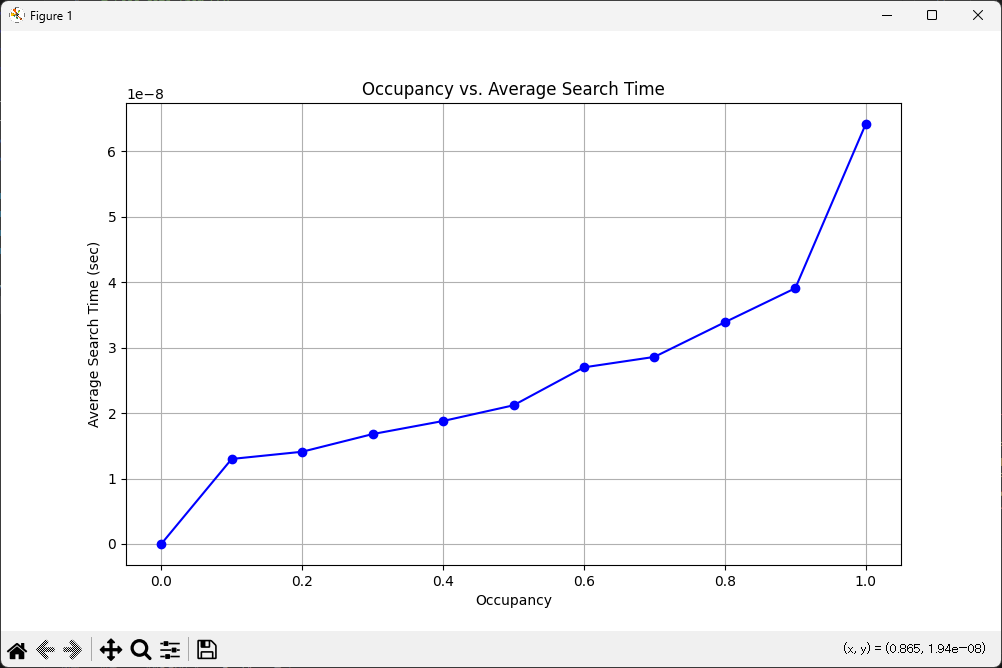
\includegraphics[width = 100mm]{searchtime.png}
\end{center}
\end{figure}
グラフを見てもやはり占有率がある程度小さい状況では時間計算量はO(1)で、占有率1.0付近で急激に増加していることが
読み取れる。これは占有率が高くなるほど再ハッシュにより探索回数が急激に増加するためだと考えられる。
\end{document}